\usetikzlibrary{arrows.meta}
\begin{figure}[htb]
\centering
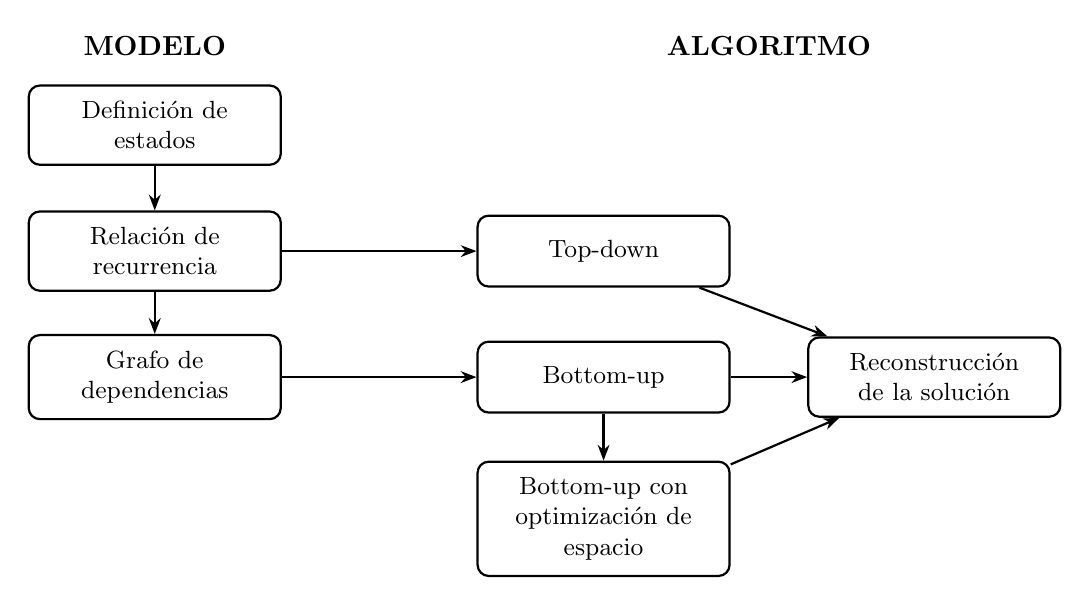
\begin{tikzpicture}[
    font=\small,
    x=1mm, y=1mm,
    box/.style={
        rectangle, draw, thick, rounded corners,
        align=center, minimum width=32mm, minimum height=9mm,
        inner sep=2mm
    },
    header/.style={font=\bfseries},
    conn/.style={-{Stealth[length=2mm]}, thick},
]

    % Column x-coordinates: a wide gap separates MODELO from ALGORITMO;
    % a narrow gap keeps the two ALGORITMO subcolumns visually grouped.
    \def\xModelo{0}
    \def\xEstrategia{57}
    \def\xReconstruccion{99}

    % Row y-coordinates.
    \def\yUno{0}
    \def\yDos{-16}
    \def\yTres{-32}
    \def\yCuatro{-50}

    % ---------- MODELO (left column) ----------
    \node[box] (estados) at (\xModelo, \yUno) {Definición de\\estados};
    \node[box] (recurrencia) at (\xModelo, \yDos) {Relación de\\recurrencia};
    \node[box] (grafo) at (\xModelo, \yTres) {Grafo de\\dependencias};

    \draw[conn] (estados) -- (recurrencia);
    \draw[conn] (recurrencia) -- (grafo);

    % ---------- ALGORITMO: estrategia de evaluación ----------
    \node[box] (topdown) at (\xEstrategia, \yDos) {Top-down};
    \node[box] (bottomup) at (\xEstrategia, \yTres) {Bottom-up};
    \node[box] (bottomup-opt) at (\xEstrategia, \yCuatro) {Bottom-up con\\optimización de\\espacio};

    \draw[conn] (recurrencia) -- (topdown);
    \draw[conn] (grafo) -- (bottomup);
    \draw[conn] (bottomup) -- (bottomup-opt);

    % ---------- ALGORITMO: reconstrucción ----------
    \node[box] (reconstruccion) at (\xReconstruccion, \yTres) {Reconstrucción\\de la solución};

    % Three independent straight arrows: each strategy reaches
    % reconstrucción directly, with no shared junction between them.
    \draw[conn] (topdown) -- (reconstruccion);
    \draw[conn] (bottomup) -- (reconstruccion);
    \draw[conn] (bottomup-opt) -- (reconstruccion);

    % ---------- Headers ----------
    \node[header] (modelo-header) at (\xModelo, 10) {MODELO};
    \node[header] (algoritmo-header) at ({(\xEstrategia+\xReconstruccion)/2}, 10) {ALGORITMO};

\end{tikzpicture}
\caption{Elementos del modelo de un problema de programación dinámica y del algoritmo que lo resuelve, incluyendo la reconstrucción de la solución.}
\label{fig:programacion_dinamica_reconstruccion}
\end{figure}
